\documentclass{book}
\usepackage[margin=1.5cm]{geometry}
\usepackage{hyperref}
\usepackage{graphicx}

\graphicspath{{./img/}}

\title{Sistemi Informativi 2022/2023}
\author{Blascovich Alessio\\
    \href{mailto:alessio.blascovich@studenti.unitn.it}{alessio.blascovich@studenti.unitn.it}}
\date{}

\begin{document}
    \maketitle
    \tableofcontents
    \chapter{Concetti generali}
    \section{Prime definizioni}
    \subsection{Informatica}
    Non è altro che la scienza dell'informazione e dei calcolatori (computer science).\\
    Anche il termine \emph{sistema informativo} è di un'ampiezza analoga, non è altro che delle procedure e delle infrastrutture che supportano il fluire delle informazioni all'interno dell'azienda.\\
    I sistemi informativi sono spesso affianchi da acronimi come \emph{ICT}, \emph{IT} e \emph{TLC}.
    \subsection{Informatica aziendale}
    E' la disciplina che cerca di studiare le applicazioni dell'informatica all'interno di un azienda e l'influenza che questa ha sul sistema aziendale.\\
    Nel prosegui come azienda ci si riferirà a piccole e medie imprese (PMI).\\
    Le aree in cui l'informatica ha un effetto sull'azienda si possono dividere in macrogruppi:
    \begin{itemize}
        \item \textbf{Aiuto e guida operativi:} con procedure che guidano l'operatore, il quale viene guidato   attraverso un tool a compiere solo passaggi corretti.\\
            Questi sistemi comprendono anche le banche dati che aiutano gli impiegati a svolgere le loro ricerche e che garantiscono l'integrità dei dati.
        \item \textbf{Organizzativa:} queste nuove tecnologie introducono sempre nuovi metodi per l'organizzazione del carico di lavoro e la sua ripartizione temporale.
        \item \textbf{Di controllo:} gli eventi possono riguardare ogni ambito dalla classica gestione degli ordini alle visite dei social network aziendali.
        \item \textbf{Strategia:} la quale può essere pensata a più lungo termine grazie all'enorme mole di dati che possono essere immagazzinati e analizzati in tempi brevissimi.
    \end{itemize}
    \subsection{Sistemi informativi aziendali}
    I sistemi interni ad un'azienda possono essere più o meno complessi e costituiti da molti o pochi elementi.\\
    Essi hanno lo scopo di aiutare i processi aziendali e di fornire delle informazioni quando richieste.\\
    Il sistema informativo di un'azienda è costruito su misura e segue le esigenze dell'impresa per cui è costruito.\\
    Dipende da:
    \begin{itemize}
        \item che fenomeni l'azienda vuole rappresentrare virtualmente.
        \item in che modo si vuole che i dati vengano rappresentati quando richiesti.
        \item dal tipo di informazioni che l'azienda vuole ottenere.
    \end{itemize}
    Gli elementi possono essere usati per gestire diversi tipi di informazioni.
    \begin{itemize}
        \item \textbf{Dati:} sono la base della rappresentazione dei fenomeni che interessano all'azienda.\\
            Solitamente i dati sono sotto forma di alcune strutture che vengono mantenute organizzate e pronte a fornire i dati richieste.\\
            I dati possono essere:
            \begin{itemize}
                \item \textbf{di configurazione:} come il saldo del conto corrente aziendale.
                \item \textbf{operativi:} come le informazioni riguardanti un task di un operatore.
                \item \textbf{di supporto:} come da dove effettua una richiesta un cliente.
                \item \textbf{di stato:} come il fatturato in un determinato periodo. 
            \end{itemize}
            \item \textbf{Procedure:} specificano le azioni che permettono al sistema di essere il più coerente possibile con la realtà, permettono anche agli utenti di interagire con il sistema stesso.
            \item \textbf{Mezzi per il trattamento delle informazioni:} in questa categoria rietrano tutti i sistemi che rendono possibile l'acquisizione dei dati e la loro distribuzione.
    \end{itemize}
    Un sistema informativo può quindi essere descritto come l'insieme dei mezzi utilizzati per implemtare dell'informatica all'interno di un'azienda.\\
    Nei sistemi l'evoluzione è costante ed è influenzata da fattori:
    \begin{itemize}
        \item interni all'azienda, come la necessità di migliorare le prestazioni.
        \item esterni all'azienda, come l'imposizione delle aziende sui subfornitori.
    \end{itemize}
    Spesso le aziende apportano delle migliorie solo nei settori dove conviene di più, per cui anche l'evoluzione deve avvenire in modo armonico con i settori meno evoluti.
    
    \section{Impatto dell'informatica nelle aziende}
    \subsection{La conoscenza dei fenomeni informatici}
    Quindi per "concludere" i sitemi informativi sono il mezzo con cui si diffondono le informazioni all'intero di un'azienda.\\
    Questo porta il sistema a doversi adattare alle diverse necessità di ogni persona.
    \begin{itemize}
        \item \textbf{Livello di astrazione:} rappresenta il grado di sintesi delle informazioni, che possono essere \textbf{analitiche} oppure \textbf{sintetiche} ovvero ottenute elaborando più informazioni elementari.
        \item \textbf{Tempestività:} indica con quanta velocità le informazioni devono transitare all'interno di un'azienda.
        \item \textbf{Livello di copertura:} comprende la quantità di fenomeni analizzati e la loro estensione a livello temporale, alcuni operatori devono analizzare le oprazioni svolte in un breve lasso di tempo, mentre altri in uno molto largo. 
    \end{itemize}
    Il sistema informativo deve quindi fornire un accesso alle risorse nelle tempistiche e nelle forme richieste, per questo le informazioni fluiscono in due direzioni:
    \begin{itemize}
        \item \textbf{Orizzonatale:} cioè tra le varie sezioni dell'azienda sincronizzando tra di loro i processi.
        \item \textbf{Verticale:} attraverso la scala gerarchica dell'azienda, con dei flussi che elaborano i dati raccolti dalle procedure.
    \end{itemize}
    \subsection{Processi classici}
    I processi che tendono ad essere informatizzati solitamente sono quelli che attirano di più l'attenzione di un informatico che ne apporta continue migliorie.\\
    Infatti i sistemi informativi vengono migliorati con i seguenti fini:
    \begin{itemize}
        \item \textbf{Sviluppo di funzioni operative:} infatti quinformatriando si pensa all'informatica ziendale si pensa subito al ridurre la mano d'opera e automatizzare delle operazioni, quindi il sistema informativo viene adottato in primo luogo per:
        \begin{itemize}
            \item Ridurre il costo del lavoro in favore di procedure automatiche standardizzate.
            \item Migliorare i processi rendendoli più controllati e omologati.
            \item Aumentare la quantità e la qualità dei dati raccolti.
        \end{itemize}
        \item \textbf{Panificazione:} con i dati raccolti con le informazioni ottenute dai processi si possono migliorare le procedure di pianificazione.\\
            La continua raccolta di informazioni ha portato ad adottare delle potiche produttive basate su MPR 2(Manufacturing Resource Planning 2).
        \item \textbf{Controllo:} la quantità e la disponibilità sempre più veloce di dati ha portato alla definizione di controllo sempre più efficaci.\\
            Il controllo sulle infromazioni puù essere automatico e nativo oppure condotto da un responsabile con informazioni fornite dal sistema.
    \end{itemize}
    Nei processi sopraelencati il sistema informativo non viene usato solo per sostituire l'operatore umano, ma anche per prendere decisioni con un livello di sicureza più elevato.
    \subsection{Struttura aziendale italiana e estera}
    In italia, non è una novità, prevalgono le piccole e medie imprese.\\
    Troviamo prova di questa affermazione consultando i dati ISTAT che rappresentano un quadro ormai stabile con minime variazioni:
    \begin{itemize}
        \item Oltre il 99.9\% delle aziende italiane rientra nella categoria di microimprese o in quelle delle piccole-medie imprese(PMI) cioè con meno di 250 dipendenti, mentre le grandi imprese sono solo il 0.1\%.
        \item Gli impiegati delle piccole e medie imprese sono circa il 72\%, relegando la forza lavoro delle grandi imprese al 22\% del totale.
    \end{itemize}
    E' facilmente immaginabile che nelle aziende di maggior dimensione siano necessarie infrastrutture più sviluppate e che di conseguenza, hanno compiuto la transizione a sistema informativo da tempo.\\
    I sistemi proggettati per le grandi imprese poco e male si adattano alle PMI, le ultime hanno bisogno di sistemi più snelli e configurabili.\\
    Ad esempio l'azienda SAP offre \emph{S/4HANA} alle grandi aziende mentre alle PMI mette a disposizione \emph{Business One}.\\
    D'ora in poi faremo solo accenni brevi cenni alle grandi aziende e parleremo solo di PMI.
    \section{Evoluzione storica}
    \subsection{Evoluzione storca dei sistemi informativi aziendali}
    Con il passare del tempo è diventata sempre più grande la dimensione della rete e la quantita di dati che devono essere immagazzinati ed elaborati.\\
    Questa evoluzione si è ripercossa anche sui sistemi informativi aziendali, i quali hanno dovuto muoversi verso una, sempre maggiore, dematerializzazione dell hardware.\\
    Il cresente uso di IoT e di social network ha dato origine ad un'enorme mole di dati (big data) che pur essendo ad uno stato grezzo contengono importantissime informazioni, per questo motivo non possono essere trattati come dati comuni e non possono essere immagazzinati in normali database.
    \subsection{Cambiamenti organizzativi aziendali generati dall'evoluzione tecnologica}
    La sempre maggiore disponibiltà di strumenti automatici ha favorito la standardizzazione e la velocità dei processi.\\
    Simultaneamente la sempre maggiore disponibilità di dati ha generato una serie di innovazioni all'interno delle aziende.\\
    \subsubsection{Organizzazione interna}
    L'evoluzione dei sistemi informativi ha seguito lo sviluppo delle tecnologie, infatti si è arrivati a considerare la tecnologia informatica una vera e propria leva strategica a disposizione dell'azienda.\\
    I cambiamenti risultano essere ragruppabili nei seguenti:
    \begin{itemize}
        \item \textbf{Riduzione dei ruoli impegatizi:} la quantità di personale amministrativo/contabile si è di molto ridotta vista la sempre maggiore potenza e correttezza delle macchine.\\
            Questo fenomeno da prima relegato alle grandi aziende si è poi espanso anche alle PMI.
        \item \textbf{Riqualifica dei ruoli:} viene revisionato il ruolo di quasi tutti gli impiegati, da compiti esecutivi ad attività qualificanti.
        \item \textbf{Riduzione dei ruoli di supporto:} come i word processo che hanno soppiantato le macchine da scrivere o i fogli di calcolo le calcolatrici.
        \item \textbf{Revisione dei processi di front office:} ai classici processi di dialogo con i clienti si sono sostituiti strumenti telematici.\\
            Scambio di dati via internet e servizi di supporto on line.
        \item \textbf{Revisione del modello organizzativo:} l'adozione sempre maggiore di sistemi informativi ha portato a modificare l'organizzazione da \emph{per funzioni} a \emph{per processi}.
        \begin{itemize}
            \item \textbf{Organizzazione per funzioni:} una divisione dei compiti che tiene in considerazione il livello di specializzazione, si concentra sull'ottimizazione di una funzione gestita da un sistema gerarchico.
            \item \textbf{Organizzazione per processi:} l'azienda viene vista come un'unica entità che si suddivide in sottoinsiemi, i quali comunicano attraverso dei processi.\\
                Tanto più sono efficaci i processi, tanto più risulta essere armonica la comunicazione dell'azienda verso il cliente.
        \end{itemize}
        \item \textbf{Reperimento sempre più dettagliato di dati:} l' IoT ed i social hanno permesso di raccogliere una mole di dati senza precedenti, i quali vengono raffinati dalle nuove tecniche di analisi dei big data che ne estraggono informazioni sempre più utili.
    \end{itemize}
    \subsubsection{Organizzazione esterna}
    Le aziende hanno iniziato ad adottare la pratica della \emph{terziarizzazione} in cui aziende medio-grandi delegano ad aziende specializzate o a loro succursali alcune parti della lavorazione.\\
    Si inizia così a formarsi una struttura reticolare con un nucleo necessario a mantenere il controllo di una rete di partner o di succursali.

    \chapter{Struttura dell'azienda e del suo sistema informativo}
    \section{Concetto di esigenza informativa}
    La funzione principale di un sistema informativo è di interagire, aiutandi, ogni figura professionale che fa funzionare l'azienda.\\
    E' importante fare due distinzioni di ruoli:
    \begin{enumerate}
        \item \textbf{Esecutivo}
        \item \textbf{Direttivo}
    \end{enumerate}
    Queste due tipologie di ruoli hanno bisogno di informazioni diverse e quindi le informazioni verranno date in modo meno o più astratto.
    \begin{itemize}
        \item I ruoli esecutivi avranno bisogno di informazioni molto specifiche della situazione attuale.
        \item I ruoli dirigenziali invece avranno a disposizione dei dati che forniscono una visione molto più ampia ma sono più sintetici.
    \end{itemize}
    All'interno del sistema informativo aziendale devono quindi coesistere i dettagli richiesti dai ruoli operativi e la sintesi richiesta dai dirigenti.

    \subsection{Schema di Anthony}
    Come abbiamo visto cambiando di mansione cambiano anche i dati che risultano utili.\\
    Ma come si può identificare a che dipendenti vanno fornite certe informazioni?\\
    Il modello di Anthony propone di distinguere le mansioni in tre livelli, ogni livello interagisce con gli adiacenti mediante cicli di verifica delle informazioni.
    \begin{enumerate}
        \item \textbf{Direzionale strategico:} identifica gli obiettivi principali a medio-lungo termine.
        \item \textbf{Direzionale tattico:} che compie analisi economiche ponendo obbiettivi a medio termine, inoltre fornisce gli indirizzi operativi ai settori esecutivi.
        \item \textbf{Operativo:} attua i piani definiti.
    \end{enumerate}
    \begin{center}
        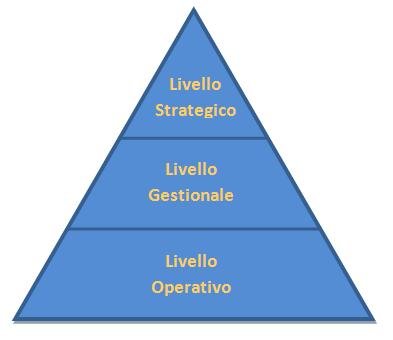
\includegraphics[scale=0.5]{anthony_mark_01.jpg}
    \end{center}

    \subsection{Profili informativi}
    \subsubsection{Livello direzionale strategico}
    A questo livello competono informazioni sintetiche, molto diversificate e poco strutturate.\\
    Al decisore deve essere affiancato un sistema informativo in grado di mostrare:
    \begin{itemize}
        \item indicatori prestazionali dell'azienda.
        \item evoluzioni delle strategie adottate in precedenza.
        \item scenari fittizzi per simulazioni.
        \item ogni tipo di indicatore sulla salute dell'azienda.
    \end{itemize}

    \subsubsection{Livello direzionale tattico}
    Il livello tattico si occupa di tutte quelle attività di definizione di obbiettivi a breve termine che rispettino le strategie aziendali e il periodico controllo dei risultati.\\
    Le informazioni necessarie sono ottenute sintetizzando i dati estratti dai sistemi di supporto al livello operativo.

    \subsubsection{Livello operativo}
    In questo livello ci si occupa dell'attuazione dei piani e delle attività correlate.

    \subsubsection{Tabella riassuntiva}
    \begin{center}
        \begin{tabular}{|l|c|c|c|c|}
            \hline
            & \textbf{Frequenza} & \textbf{Dati} & \textbf{Provenienza} & \textbf{Volumi}\\
            \hline
            \textbf{\begin{tabular}{@{}c@{}} Livello \\ direzionale \\ strategico \end{tabular}} & casuale & \begin{tabular}{@{}c@{}} sintetici e\\ non strutturati \end{tabular} & interna ed esterna & bassi\\
            \hline
            \textbf{\begin{tabular}{@{}c@{}} Livello \\ direzionale \\ tattico \end{tabular}} & prefissata & sintetici o analitici & interna & medi\\
            \hline
            \textbf{\begin{tabular}{@{}c@{}} Livello \\ operativo \end{tabular}} & costante & analitici & interna & elevati\\
            \hline
        \end{tabular}
    \end{center}

    \section{Scomposizione del sistema informativo}
    Le diverse esigenze tra i  vari livelli ha portato, nel tempo, ad una separazione tra i sistemi informativi.\\
    Si sono venuti a creare due tipologie di sistemi:
    \begin{enumerate}
        \item \textbf{Sistemi informazionali:} che aiutano nella risoluzione di problemi che non sempre hanno una struttura precisa, vengono alimentati con i dati raccolti dai sistemi operazionali.\\
            Negli anni si sono evoluti per collezioanre in modo sempre più rapido ed efficente l'andamento azziendale e quello della concorrenza.
        \item \textbf{Sistemi operazionali:} hanno una strattura fissa e molto rigida, infatti svolgono il mestiere per il quale vengono pensati, non sono più di aiuto quando si voglia percorrere un percorso di risoluzione diverso.
    \end{enumerate}
    \begin{center}
        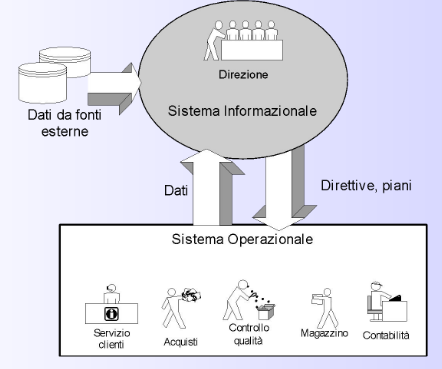
\includegraphics[scale=0.6]{relazione_sistemi_operazionale_informazionale.png}
    \end{center}
    Questa separazione rompe però la struttura di Anthony che può essere riopensata come:
    \begin{center}
        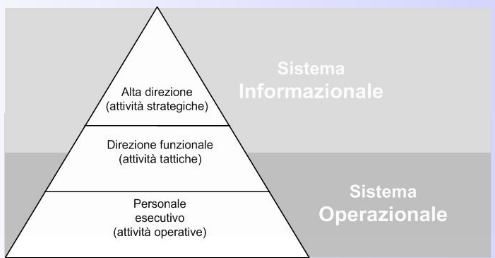
\includegraphics[scale=0.5]{anthony_mark_02.png}
    \end{center}
\end{document}